\section{Поправка на смещение}

Зачем нам нужно оценивать смещение $\hat{\theta}$? Обычная причина --- исправить $\hat{\theta}$, чтобы она стала менее смещенной. Если $\widehat{\text{bias}}$ является оценкой смещения $\text{bias}_{F}(\hat{\theta}, \theta)$, то очевидной оценкой с поправкой на смещение является
\begin{equation}\label{eq10.40}
    \bar{\theta} = \hat{\theta} - \widehat{\text{bias}}
\end{equation}
Принимая $\widehat{\text{bias}}$ равным $\widehat{\text{bias}}_{B} = \hat{\theta}^{*}(\cdot) - \hat{\theta}$, получаем
\begin{equation}\label{eq10.41}
    \Bar{\theta} = 2\hat{\theta} - \hat{\theta}^{*}(\cdot).
\end{equation}
(Существует тенденция --- неправильная тенденция --- думать о самой $\hat{\theta}^{*}(\cdot)$ как о скорректированной на смещение оценке. Обратите внимание, что (\ref{eq10.41}) показывает, что если $\hat{\theta}^{*}(\cdot)$ больше $\hat{\theta}$, то исправленная оценка $\Bar{\theta}$ должна быть меньше $\hat{\theta}$.) Положим $\widehat{\text{bias}} = 0.0080$ для статистики отношения данных об уровне гормона при ношении пластырей, равной как $\overline{\text{bias}}_{400}$, так и $\widehat{\text{bias}}_{\text{jack}}$, исправленная оценка отношения $\theta$ равна
\begin{equation}\label{eq10.42}
    \Bar{\theta} = -0.0713 - 0.0080 = -0.0793. 
\end{equation}

На практике исправление смещения может быть опасным. Даже если $\Bar{\theta}$ менее смещена, чем $\hat{\theta}$, она может иметь значительно большую стандартную ошибку. Еще раз, это можно проверить с помощью бутсрепа. Для статистики отношения данных об уровне гормона $200$ бутстреп репликаций $\Bar{\theta} = \hat{\theta} - \widehat{\text{bias}}_{\text{jack}}$ сравнивались с соответствующими репликациями $\hat{\theta}$. Бустреп оценки стандартной ошибки $\bar{\theta}$ и $\hat{\theta}$ были почти идентичны, поэтому в этом случае исправление смещения не было опасным.

\noindent
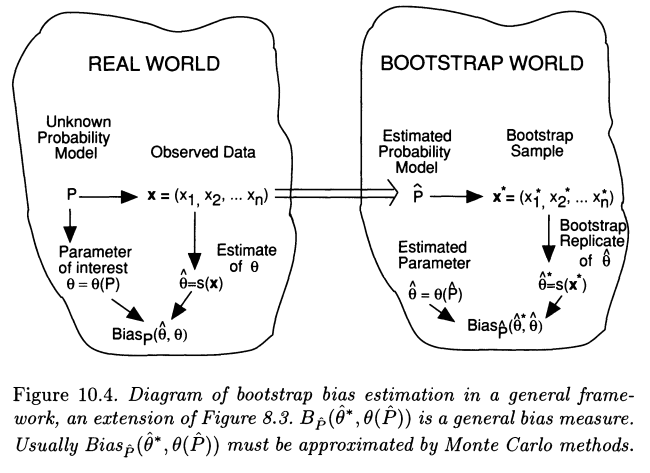
\includegraphics[width=\linewidth]{10/f10.4.png}
\newline

Подводя итог, можно сказать, что оценка смещения обычно интересна и целесообразна, но точное использование оценки смещения часто проблематично. Систематические ошибки оценить труднее, чем стандартные ошибки, как показано на рисунке 10.3. Прямое исправление смещения (\ref{eq10.40}) может быть опасно для использования на практике из-за большой изменчивости $\widehat{\text{bias}}$. Исправление смещения может вызвать большее увеличение стандартной ошибки, что, в свою очередь, приводит к большей среднеквадратичной ошибке (уравнение (\ref{eq10.14})). Если $\widehat{\text{bias}}$ мало по сравнению с предполагаемой стандартной ошибкой $\widehat{\text{se}}$, то безопаснее использовать $\hat{\theta}$, чем $\Bar{\theta}$. Если $\widehat{\text{bias}}$ велико по сравнению с $\widehat{\text{se}}$, то это может указывать на то, что статистика $\hat{\theta} = s(x)$ не является подходящей оценкой параметра $\theta$.

Оценка ошибки предсказания --- одна из важных задач, в которой полезно исправление смещения. Смещение очевидной оценки велико по сравнению со стандартной ошибкой, и его можно эффективно уменьшить, добавив поправочный член. Подробности приведены в главе 17.